% !TEX root = ../main.tex

% 结语部分
\section{ET2-1 Welding and Debugging of Bluetooth Speakers \\ The End}


%---------------------------------------------------------------------
% 总结、杂谈与致谢
\subsection{Summary, Thoughts \& Acknowledgments}
\begin{enumerate}
	\item Thank you, teacher, for taking the time to read this experimental report, which still has many shortcomings. I hope you can point out the areas that need improvement. I wish you good health, happiness in life, and success in your work!
	\item Through this experiment, we consolidated the theoretical analysis method and experimental measurement method of circuit magnification learned in electronic technology class, basically mastered the use of soldering iron, and learned KiCAD tool by ourselves.
\end{enumerate}


%---------------------------------------------------------------------
% 附件
\subsection{Attachment}
%The arrangement of the experimental bench desktop is shown in %\cref{}.

The personal signature of the experimental report is shown in \cref{fig:name1} and \cref{fig:name2}.

\begin{figure}[htbp]
	\centering
	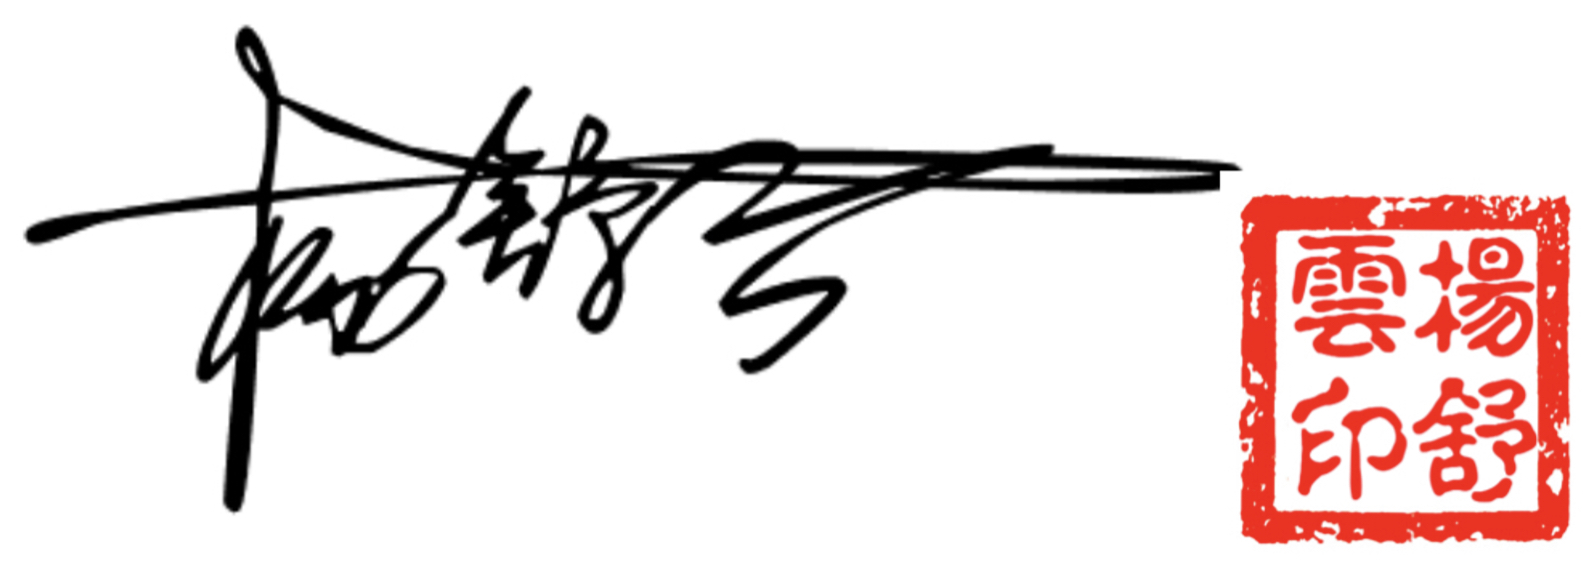
\includegraphics[width=0.5\textwidth]{name.png}
	\caption{signature1}
	\label{fig:name1}
\end{figure}

\begin{figure}[htbp]
	\centering
	
\includegraphics[width=0.35\textwidth]{name-TaLEs.jpg}
	\caption{signature2}
	\label{fig:name2}
\end{figure}

\textbf{All relevant code (Python and LaTex source code) has been uploaded to Github.}


%---------------------------------------------------------------------
% 参考文献
\renewcommand{\refname}{Reference}
\begin{thebibliography}{99}	
	\bibitem{a} 维基百科. \emph{维基百科}[M]. https://zh.wikipedia.org
	\bibitem{b} 沈韩. \emph{基础物理实验}[M]. 北京: 科学出版社, 2015.	
\end{thebibliography}